\section{Supplementary Methodology}
\subsection{Pre-Transformation Module} \label{app:trans}
Let us review the process of computing the separability $\theta_{i,j}$. Given a feature pair $(f_i,f_j)$ and the corresponding positive and negative centroids, {\em (i)} we first compute $w_0$, $w_i$ and $w_j$ for $\lhat$\eat{ based on Equation~\ref{eqn:rep_line}}. Next, for each object $o_k$, {\em (ii)} we obtain the predicted label $\eta_{i,j}^{\lhat,k}$ according to Equation~\ref{eqn:est_label}. This step requires two multiplications and three additions. Finally, {\em (iii)} we calculate $\theta_{i,j}^{k}$ and the separability $\theta_{i,j}$ based on Equations in Section~\ref{sec:metric}\eat{Equation~\ref{eqn:s_object} and \ref{eqn:s_line} respectively}. This whole process is repeated for every feature pair candidate. However, there is massive redundancy across the processing of different feature pairs. For instance, when calculating the separability for two different feature pairs $(f_i,f_j)$ and $(f_i,f_{j'})$ with a common $f_i$, $w_i$ is in fact shared, and calculation of $w_i\cdot \mm_{i,k}$ in Equation~\ref{eqn:est_label} is repeated for each object $o_k$.
\tr{\sinha{is there another work we can cite that has done this?} \silu{Aditya's another paper~\cite{parameswaran2012crowdscreen} did similar trick, but in different problem. Do we want to cite it?}\agp{I think it's too far off.}}

Given this, we propose the \trans optimization module which will pre-calculate some common computational components once across different features and reuse these components the separability for each feature pair to eliminate the repeated computation. This \trans module transforms the original $\mm_{i,k}$ matrix into another space using our identified common feature pair components and updates the separability score equation accordingly.

For each feature $f_i$, we find the average values of the positive and negative objects for that feature, $\mm_i^+$ and $\mm_i^-$ respectively, and then we pre-transform $\mm_{i,k}$, i.e., the value of object $o_k$ on the feature $i$, to $\widehat{\mm}_{i,k}=$ $\Big( (\mm_i^+-\mm_i^-)\cdot \mm_{i,k}-\frac{(\mm_i^+)^2-(\mm_i^-)^2}{2} \Big) \cdot l_k$.
\eat{
\begin{equation}\label{eqn:matrix_transform}
\widehat{\mm}_{i,k} = \Big( (\mm_i^+-\mm_i^-)\cdot \mm_{i,k}-\frac{(\mm_i^+)^2-(\mm_i^-)^2}{2} \Big) \cdot l_k
\end{equation}
}
The basic idea is to decompose
Equation~\ref{eqn:est_label} into two components,
with each one only related to a single feature.
This transformation incorporates
the class centroids into the matrix values,
obviating their integration later
for every feature pair that involves the given feature.
We\eat{Equation~\ref{eqn:matrix_transform}} also multiplies
in the class label of the object, $l_k$,
rather than repeating this multiplication every time the object is evaluated (see example in \transfig). With this transformation of the feature-object matrix,
evaluating whether an object was correctly separated is simplified as: if $sign(\widehat{\mm}_{i,k} + \widehat{\mm}_{j,k}) = 1$, then $\theta_{i,j}^{k}=1$; otherwise, $\theta_{i,j}^{k}=0$. \eat{from Equation~\ref{eqn:s_object} into Equation~\ref{eqn:s_object_transform}:
% \agp{confusing because $L$ is not there in Equation~\ref{eqn:s_object}}\silu{maybe add "Since our focus is on Rocchio-based measure, we replace the separating line $\ell$ in Equation~\ref{eqn:s_object} with the representing line $L$ in Equation~\ref{eqn:s_object_transform}."}
%, and get rid of checking the real label $l_k$ in Equation~\ref{eqn:s_object}
\begin{equation}\label{eqn:s_object_transform}
\theta_{i,j}^{k}=\left\{
 \begin{array}{ll}
  1 \textit{\hspace{2mm} if \hspace{2mm}} sign(\widehat{\mm}_{i,k} + \widehat{\mm}_{j,k}) = 1\\
  0 \textit{\hspace{2mm} otherwise \hspace{2mm}}
 \end{array}
 \right.
\end{equation}
%\begin{equation}\label{eqn:est_label_transform}
%\eta_{i,j}^{\lhat,k}=\sign(\widehat{\mm}_{i,k} + \widehat{\mm}_{j,k})
%\end{equation}
After pre-transformation, we are now ready
to compute the separability score $\theta_{i,j}$.
Given a feature pair $(f_i,f_j)$, we can compute $\theta_{i,j}^{k}$
for each object $o_k$ based on Equation~\ref{eqn:s_object_transform}.}
Note that this step only involves one addition and one comparison and is performed only once for each feature.
Next, we can calculate overall separability score $\theta_{i,j} = \sum_{k}{\theta_{i,j}^{k}}$\eat{ like in Equation~\ref{eqn:s_line} without the pre-transformation}. Overall,
we not only eliminate the steps of computing
$w_0$, $w_i$ and $w_j$ for every feature pair,
but also reduce the cost of calculating
$\eta_{i,j}^{k}$ in Equation~\ref{eqn:est_label}.
In the following sections,
we will consider $\widehat{\mm}$ using pre-transformation instead of $\mm$, and calculate $\theta_{i,j}$ accordingly\eat{
and Equation~\ref{eqn:s_object_transform} instead of
Equation~\ref{eqn:est_label} and~\ref{eqn:s_object}}.
%Hence, by conducting transformation in Equation~\ref{eqn:matrix_transform} and~\ref{eqn:s_object_transform}, we have mapped our problem to a new space.

%\begin{figure}[h]
%\centering %%% not \center
%\vspace{-2mm}
%\subfigure[Pre-Transformation]{\label{fig:transform}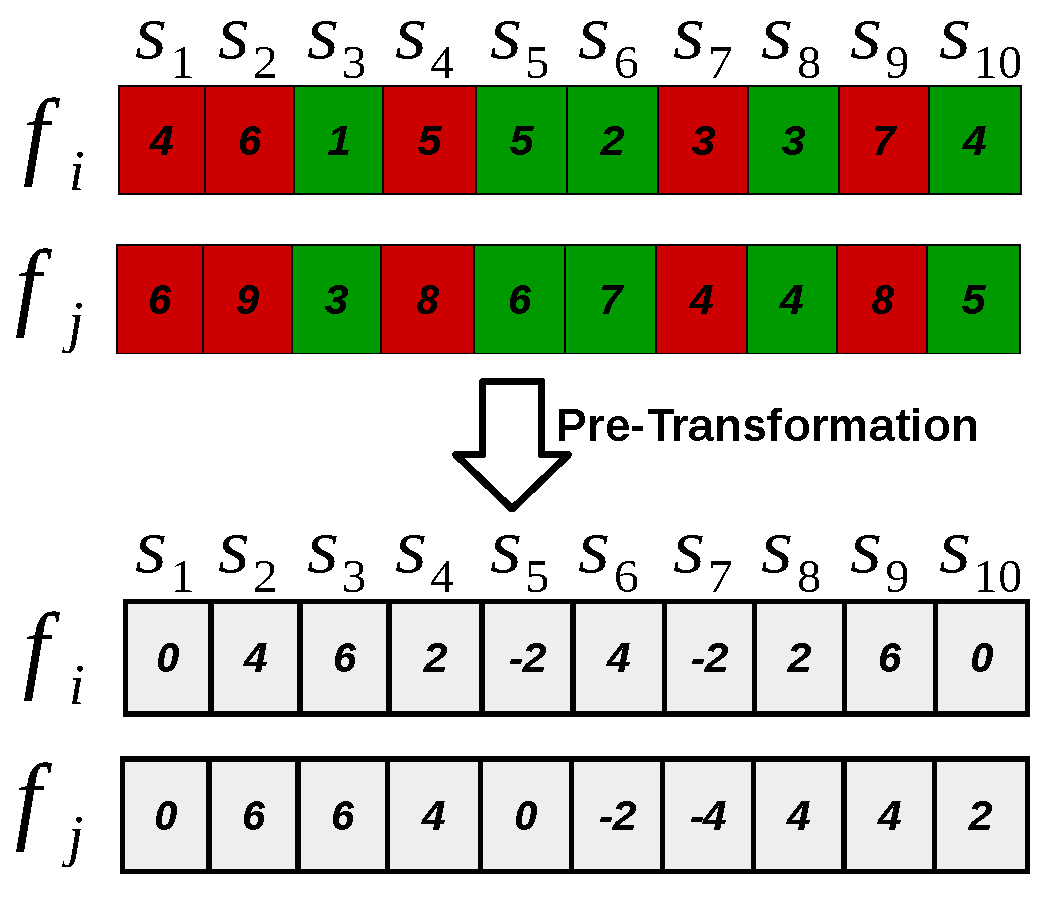
\includegraphics[width=.235\textwidth]{fig/transformation.pdf}}
%\subfigure[Early Termination ($\tau = 1$)]{\label{fig:earlyT}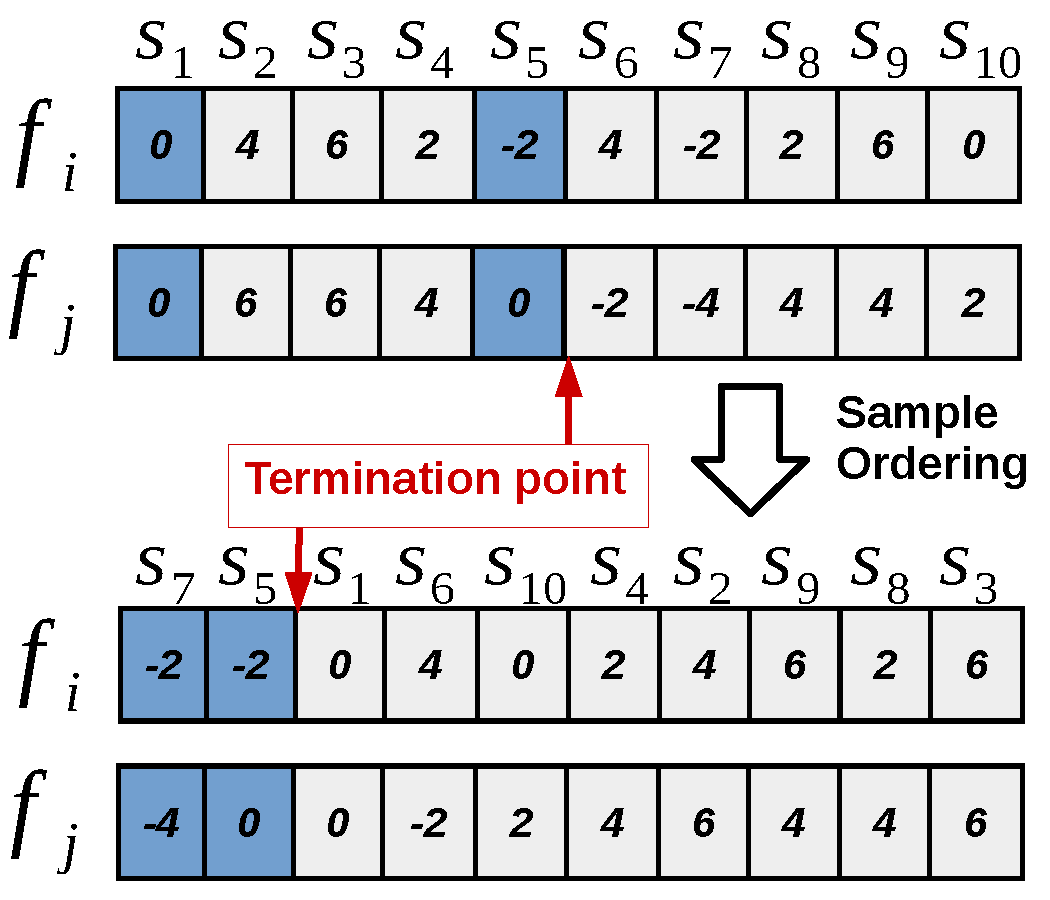
\includegraphics[width=.235\textwidth]{fig/earlyT.pdf}}
%\vspace{-5mm}
%\caption{Optimizations for Feature Pair Evaluation. (a) The \trans module is applied once to the original values in the feature-object matrix $\mm$ (above) using Equation~\ref{eqn:matrix_transform} to produce $\widehat{\mm}$ (below). (b) With the \earlyT module, a feature pair can be discarded from consideration for the \topk before all objects are evaluated (above) with even greater speedup potential after re-ordering the objects (below).}
%\vspace{-8mm}
%\label{fig:trans_term}
%\end{figure}

%\begin{example}[Transformation]
%Figure~\ref{fig:transform} illustrates the transformation for two features, $f_i$ and $f_j$. The top half depicts $\mm_{i,k}$ and $\mm_{j,k}$ before transformation, where green color represents a positive label and red color represents a negative label. In this example, the centroids of the positive and negative objects are $\mu_{i,j}^+=(5,7)$ and $\mu_{i,j}^-=(3,5)$ respectively. Hence, we can rewrite Equation~\ref{eqn:matrix_transform} as $\widehat{\mm}_{i,k} = (2\mm_{i,k}-8)\cdot l_k$ and $\widehat{\mm}_{j,k} = (2\mm_{i,k}-12)\cdot l_k$ for features $f_i$ and $f_j$ respectively. After calculation, we can obtain the values for $\widehat{\mm}_{i,k}$ and $\widehat{\mm}_{j,k}$ shown in the bottom half of Figure~\ref{fig:transform}.
%\end{example}

%%%%%%%%%%%%%%%%%%%%%%%%%%%%%%%%%%NEED TOGGLE%%%%%%%%%%%%%%%%%%%%%%
% \begin{figure}[h]
% \centering
% \begin{subfigure}{0.235\textwidth}
% \centering
% 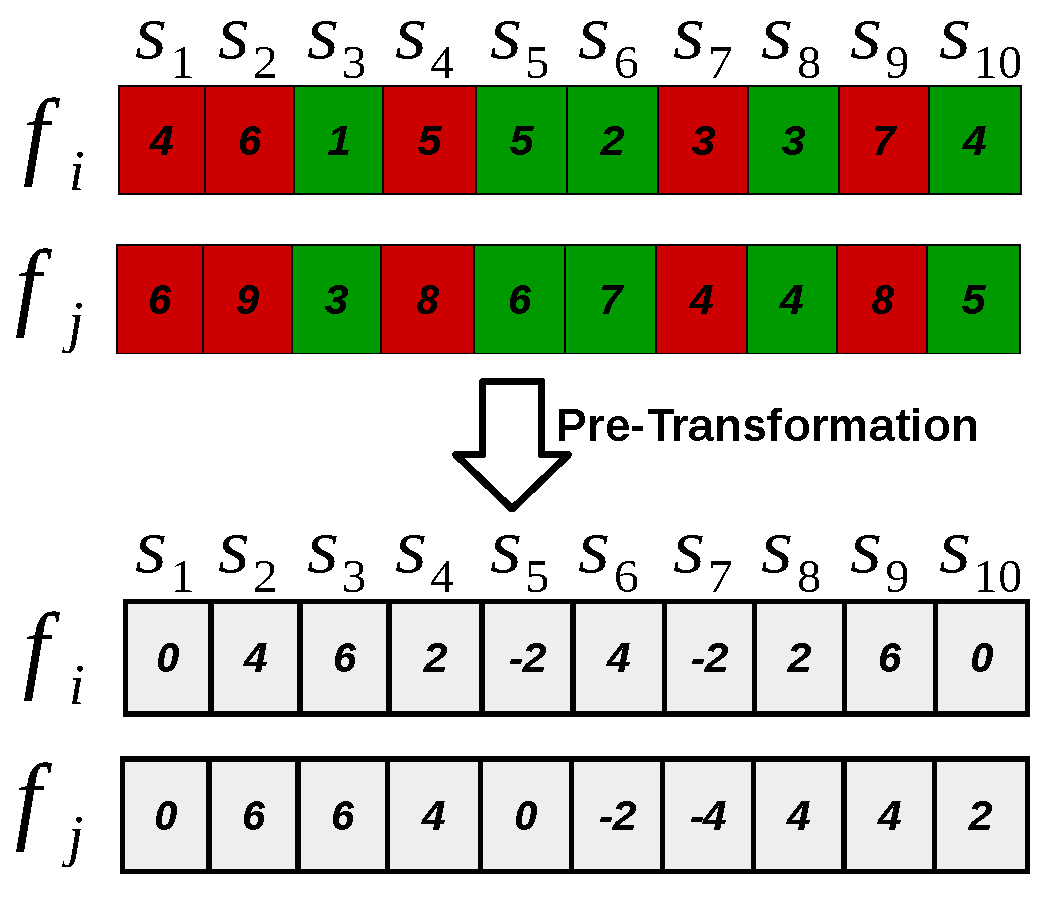
\includegraphics[width=\linewidth]{fig/transformation.pdf}
% \vspace{-5mm}
% \caption{Pre-Transformation}%{$\theta_{i,j}^{\ell}$ with Different Lines}
% \label{fig:transform}
% \end{subfigure}
% \begin{subfigure}{.235\textwidth}
% \centering
% 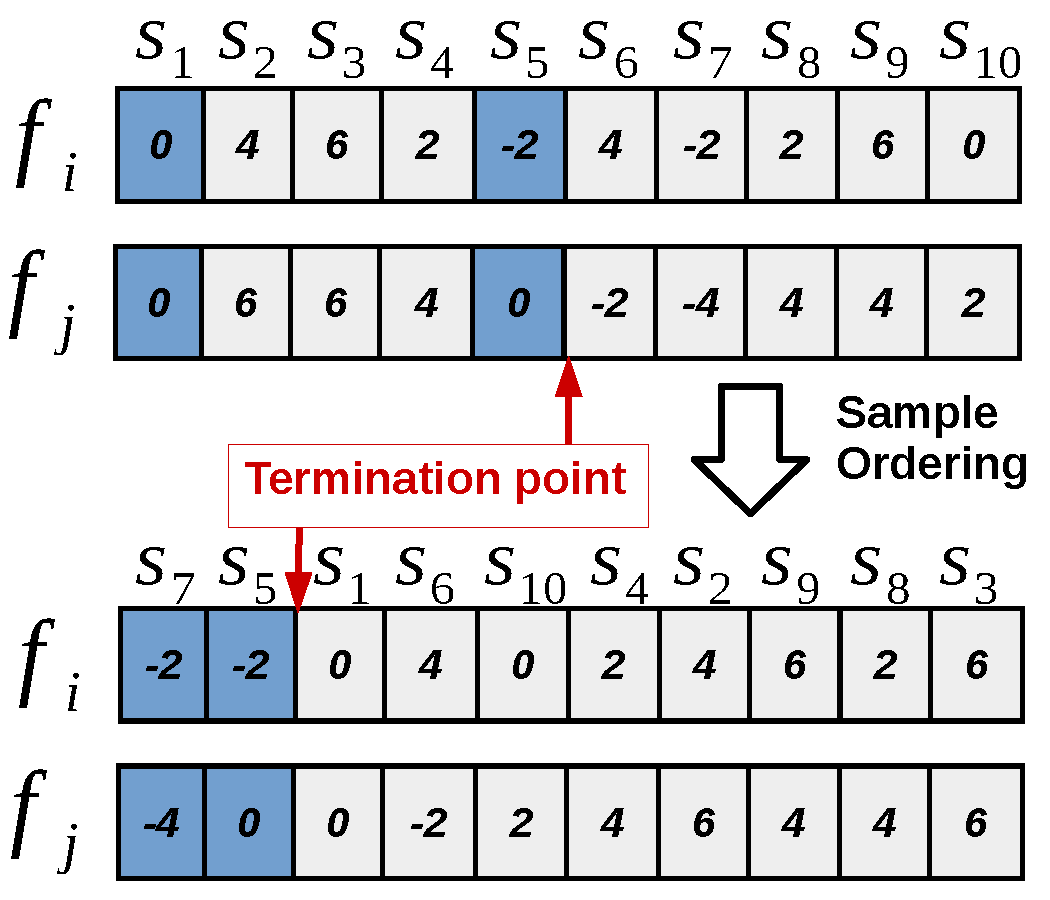
\includegraphics[width=\linewidth]{fig/earlyT.pdf}
% \vspace{-5mm}
% \caption{Early Termination ($\tau = 1$)}%{$\theta_{i,j}^{\lhat}$ with Representative Line}
% \label{fig:earlyT}
% \end{subfigure}
% \caption{Different Methods to Reduce Running Time}
% \label{fig:metric}
% \end{figure}


\subsection{Sample Size in \sampling} \label{app:sampling}
We have proposed \sampling for estimating $\theta_{i,j}$ in Section~\ref{ssec:sampling}. Next, we formally quantize the sample set size in Theorem~\ref{them:est}.

\begin{theorem}[Estimation Accuracy]\label{them:est}
By considering $\Omega(\frac{1}{\epsilon^2}\cdot \log(\frac{1}{\delta}))$ samples, with probability at least $1-\delta$, we have $|\frac{\theta_{i,j}(\sss)}{|\sss|}-\frac{\theta_{i,j}}{n}| \leq \epsilon$, i.e., $|\tilde{\theta}_{i,j}-\theta_{i,j}|\leq \epsilon n$.
\end{theorem}
\tr{\begin{proof}
  Based on Hoeffding's inequality:
  $$Pr(|\frac{\theta_{i,j}(\sss)}{|\sss|}-\frac{\theta_{i,j}}{n}| \geq \epsilon) \leq 2e^{-2|\sss|\epsilon^2}$$
  Hence, when $|\sss| = \frac{1}{2\epsilon^2}\cdot \log(\frac{2}{\delta}) = \Omega(\frac{1}{\epsilon^2}\cdot \log(\frac{1}{\delta}))$, we have:
$$
  Pr(|\frac{\theta_{i,j}(\sss)}{|\sss|}-\frac{\theta_{i,j}}{n}| \geq \fepsilon) \leq \delta \ \ \ \ \ \ \ \ \ \ \ \square
$$
\end{proof}
}
\noindent We can treat $\log(1/\delta)$ as a constant, e.g., by setting $\delta = 0.05$. Thus, Theorem~\ref{them:est} essentially states that with only $\Omega(\frac{1}{\epsilon^2})$ samples, with probability 95\%, the confidence interval for $\theta_{i,j}$ is $[\tilde{\theta}_{i,j}-\epsilon n, \tilde{\theta}_{i,j}+\epsilon n]$. 

\subsection{Example of \traversal} \label{app:trav}
Assume $m=2\times 10^4$. Initially, the number of possible feature pairs is roughly $\frac{m^2}{2}=2\times 10^8$. However, if we limit the number of considered feature pairs to $\chi=10^7$, we reduce our search space to $\frac{1}{20}$ of the total number of feature pairs. We order the single features by their individual separability scores. In horizontal traversal, only feature pairs with at least one individual feature ranked in the top 500 will be considered; while vertical traversal will consider only feature pairs with both individual features ranked better than 2000.

\section{Supplementary Table}

\subsection{Details for Running Time Comparison}\label{appT:time}
For each dataset collection, MSigDB and LINCS, show two statistics FPsChecked and ObjectsChecked, for each optimization module phase (columns).  FPsChecked is the number of feature pairs evaluated in the phase, and ObjectsChecked is the average number of sample objects that are evaluated accross all feature pairs.

\subsection{Detailed Analysis of 'Improved' Feature Pairs}\label{appT:fp}
For each drug dataset (col C), we return a limited number of gene feature pairs (cols E,F) that after correction were the most "improved" over their corresponding single feature results either by the change in the corrected\_pvalue (cols H,I,J,N,O) or the change in the feature rankings (cols K,L,M,P).  Pubmed IDs (cols Q,R) are provided when the relationship between the drug and the gene feature were found in the Comparative Toxicogenomics Database (CTD) or by manual literature search (denoted by *-asterisk).  When relationships between the gene features themselves were discovered, the type and strength of the relationships were reported (col S) and the number of relationships quantified (col T).

\subsection{Notations in the Paper}~\label{appT:notation}
\begin{table}[h]
\centering
\small
\begin{tabular}{|c|c|c|c|}
 \hline
 Symb. & Description & Symb. & Description\\
 \hline
 \hline
 $\mm$ & feature-object matrix & $\ff$ & feature set in $\mm$ \\
 \hline
 $f_i$ & feature $i$ in $\ff$ & $m$ & number of features in $\ff$\\
 \hline
 $\oo$ & object set in $\mm$ & $N$ & number of objects in $\oo$\\
 \hline
 $\oo_+$ & positive object set & $\oo_-$ & negative object set\\
 \hline
 $\widehat{\oo}$ & labelled object set & $n$ & number of labelled objects in $\widehat{\oo}$\\
 \hline
 $o_k$ & object $k$ in $\widehat{\oo}$ & $l_k$ & label of object $o_k$\\
 \hline
 $\ell$ & separating line in 2-D & $\lhat$ & representative line in 2-D\\
 \hline
 $\eta_{i,j}^{\ell,k}$ & predicted label of $o_k$ & $\theta_{i,j}^{\ell,k}$ & $o_k$ is correctly separated? \\
 \hline
 $\theta_{i,j}^{\ell}$ & \# correctly separated $o_k$ & $\theta_{i,j}$ & separability score\\
 \hline
 $\widehat{\mm}$ & $\mm$ after transformation & $\tilde{\theta}_{i,j}$ & estimated $\theta_{i,j}$\\
 \hline
 \end{tabular}
\caption{Notation used in this paper.}
\label{tbl:notation}
\vspace{-18pt}
\end{table}

\section{Supplementary Figure}
\subsection{\trans}~\label{appF:transform}
\begin{figure}[h]
\centering %%% not \center
\vspace{-6mm}
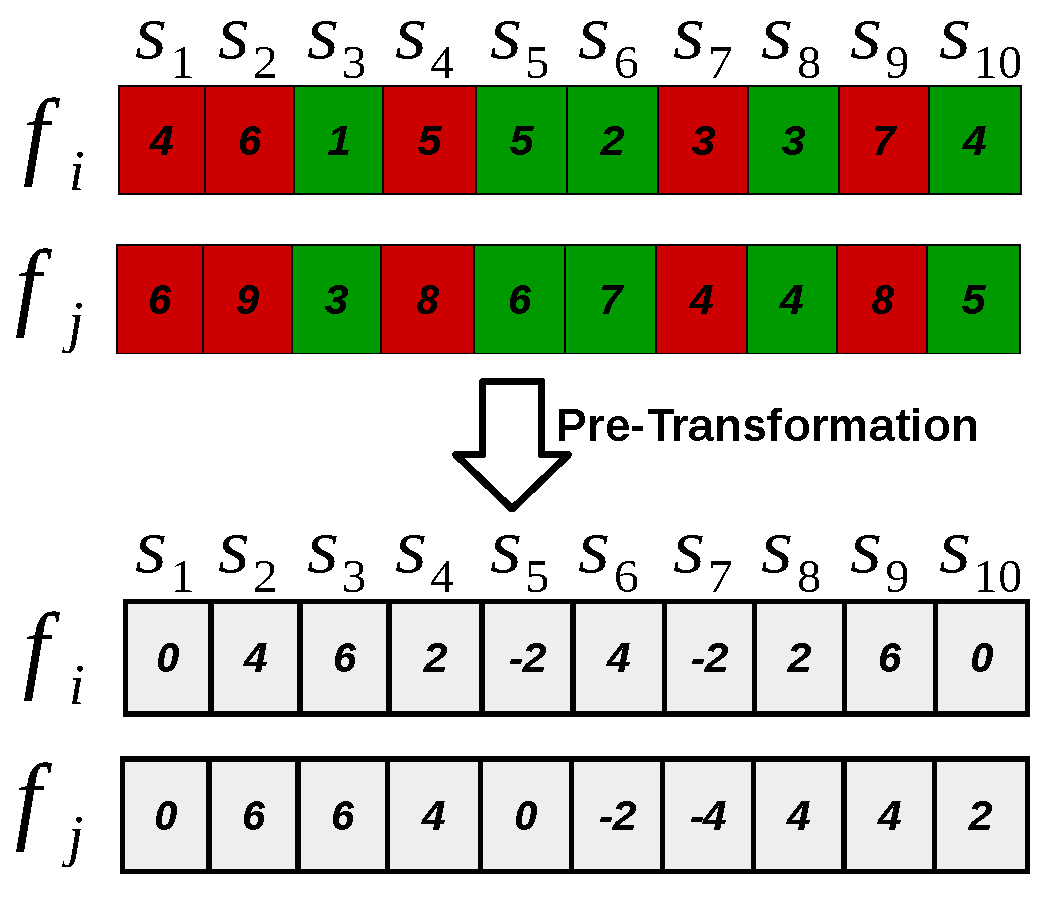
\includegraphics[width=.235\textwidth]{fig/transformation.pdf}
\vspace{-5mm}
\caption{The \trans module is applied once to the original values in the feature-object matrix $\mm$ (above) to produce $\widehat{\mm}$ (below). For two features, $f_i$ and $f_j$. The top half depicts $\mm_{i,k}$ and $\mm_{j,k}$ before transformation, where green color represents a positive label and red color represents a negative label. In this example, the centroids of the positive and negative objects are $\mu_{i,j}^+=(5,7)$ and $\mu_{i,j}^-=(3,5)$ respectively. Hence, we can rewrite $\widehat{\mm}_{i,k} = (2\mm_{i,k}-8)\cdot l_k$ and $\widehat{\mm}_{j,k} = (2\mm_{i,k}-12)\cdot l_k$ for features $f_i$ and $f_j$ respectively. After calculation, we can obtain the values for $\widehat{\mm}_{i,k}$ and $\widehat{\mm}_{j,k}$ shown in the bottom half.}
\vspace{-8mm}
\label{fig:trans_term}
\end{figure}


\subsection{\traversal}~\label{appF:traversal}
\begin{figure}[h]
 \centering
 \vspace{-5mm}
 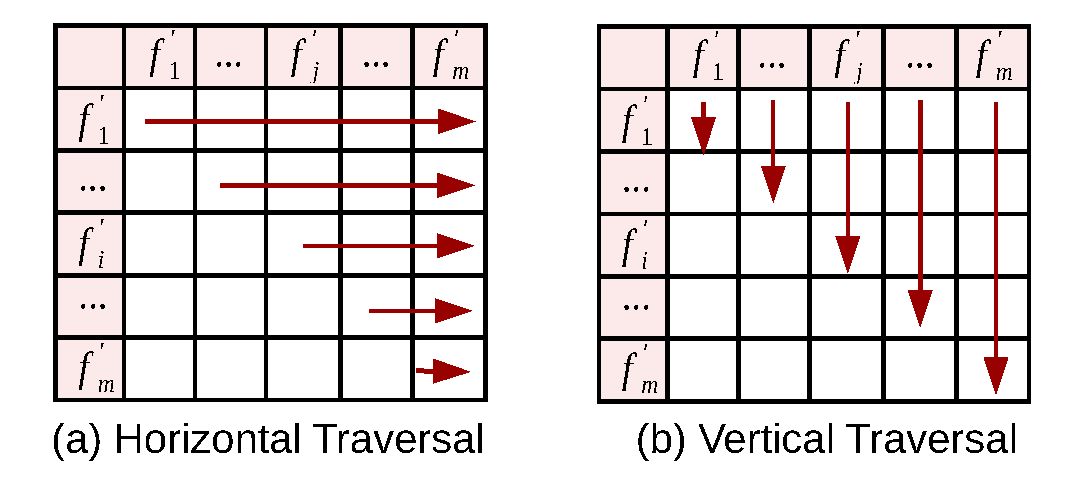
\includegraphics[width=0.7\linewidth]{fig/traversal.eps}
 \vspace{-5mm}
\caption{After feature ordering, \traversal enables \genviz is able to examine the feature pair search space (a) horizontally or (b) vertically.}
\vspace{-5mm}
\label{fig:traversal}
\end{figure}

\subsection{Separability Score Comparison}~\label{appF:exp_sep}
\begin{figure}[h]
\centering %%% not \center
\vspace{-5mm}
\subfigure[Best Feature Pair Comparison]{\label{fig:brute_rocchio_ratio}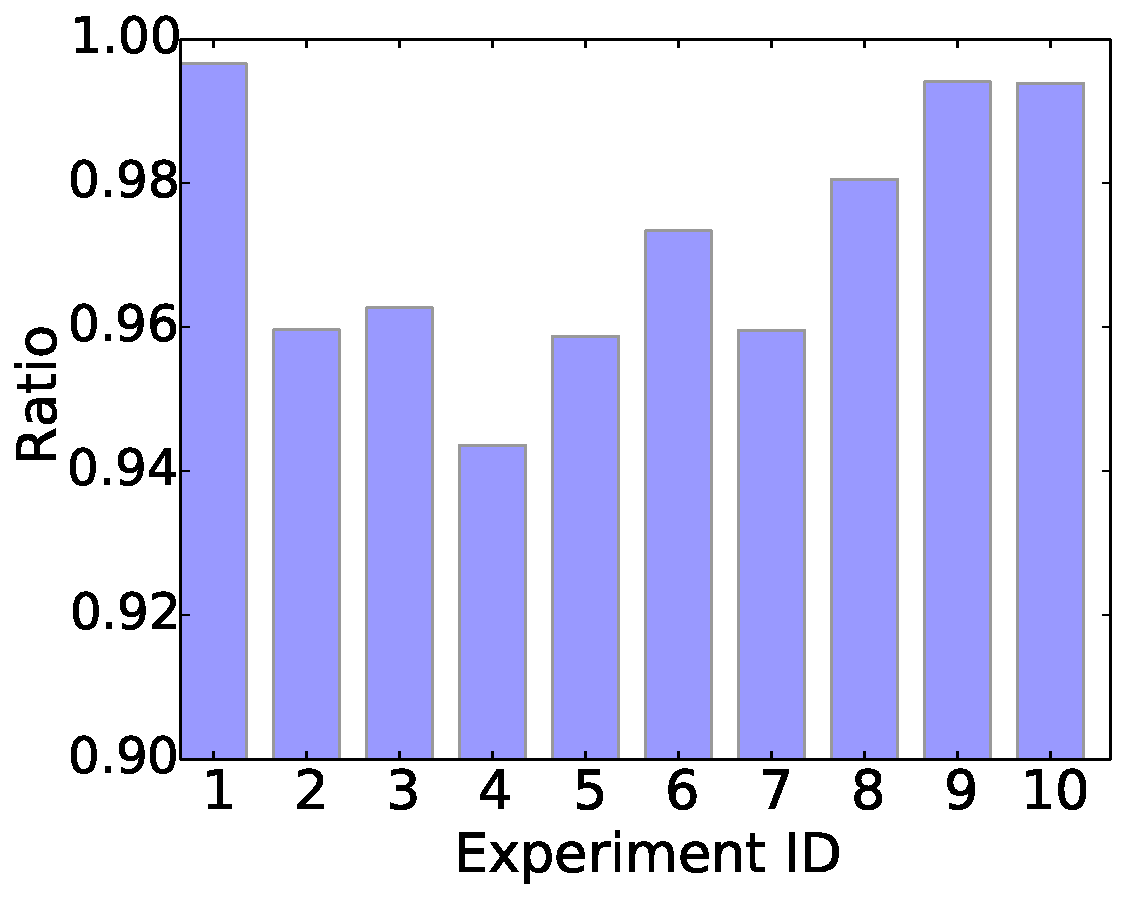
\includegraphics[width=.235\textwidth]{fig/rocchio_brute_ratio.pdf}}
\subfigure[Measure Comparison]{\label{fig:brute_rocchio_score}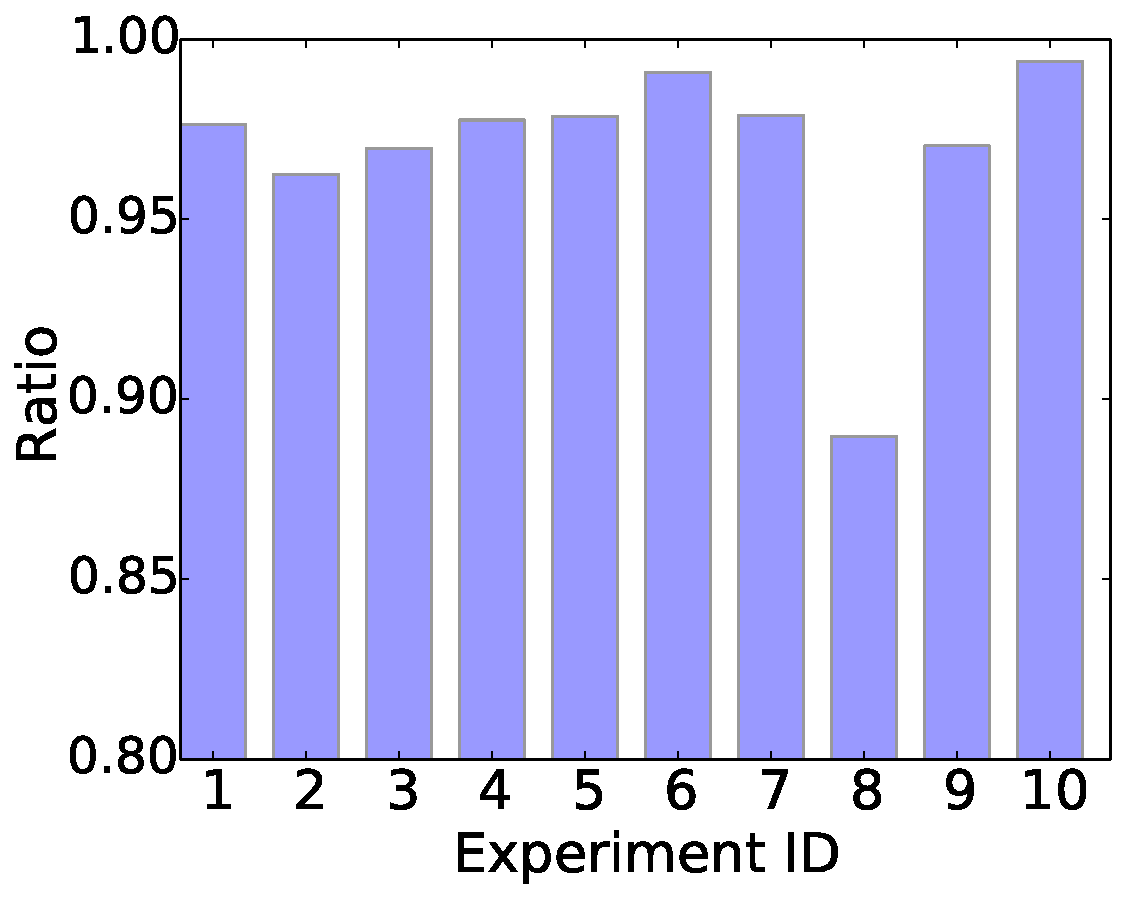
\includegraphics[width=.235\textwidth]{fig/rocchio_brute_score.pdf}}
\vspace{-5mm}
\caption{Comparison of Brute Force-based and Rocchio-based separability score. (a) For each of 10 datasets, we display the ratio of the true separability score between the best feature pair chosen by brute force and by the Rocchio-based method. (b) For each dataset, we display the ratio of the true separability score and the Rocchio-based separability score for the best feature pair selected using Rocchio-based method.}
\vspace{-5mm}
\label{fig:brute_rocchio}
\end{figure}

\subsection{Histogram of $improv\_quot$}~\label{appF_exp_hist}
\begin{figure}[h]
\centering %%% not \center
\vspace{-1mm}
\subfigure[\msig]{\label{fig:msig_histogram_diff}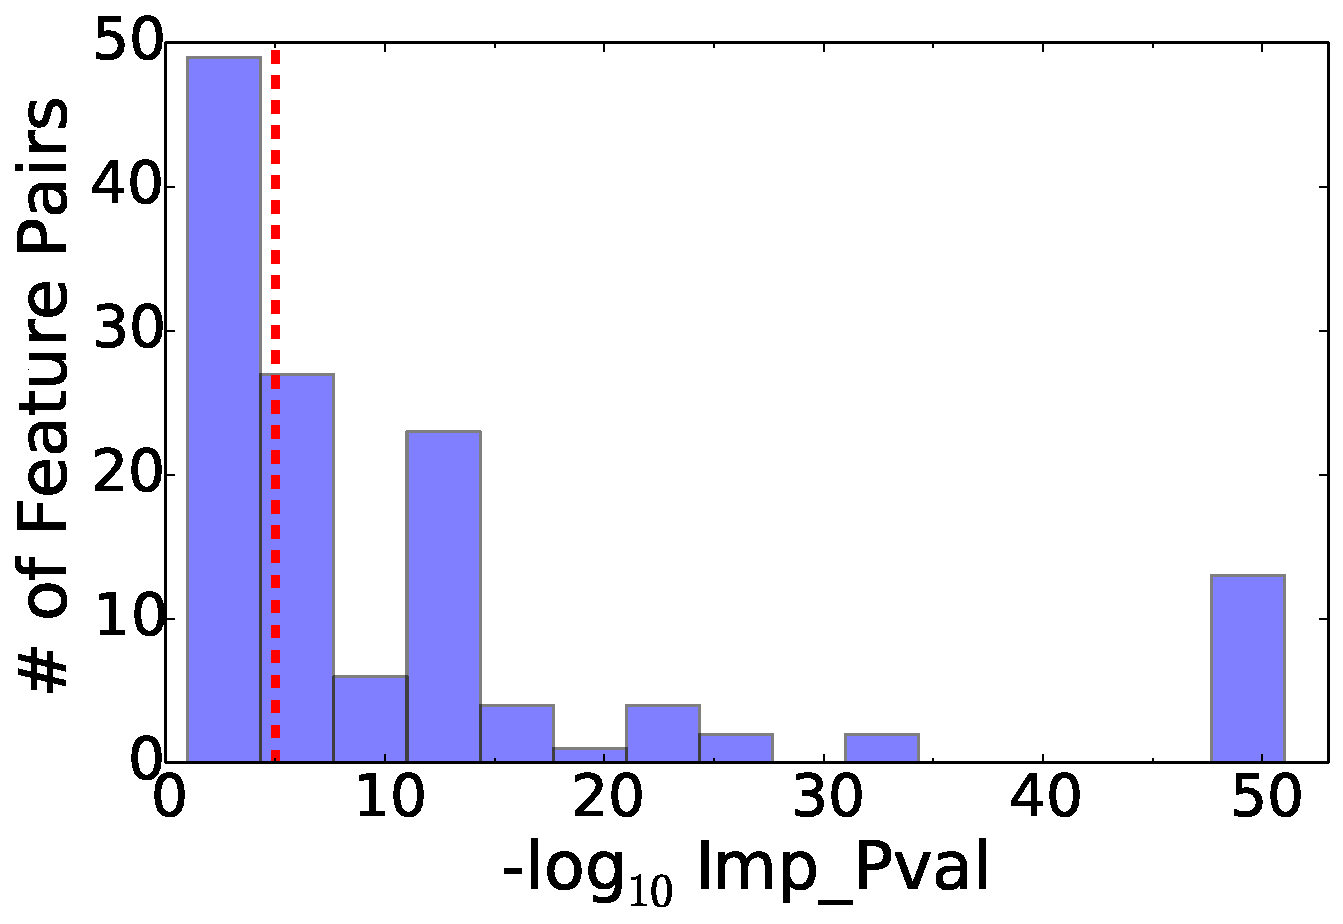
\includegraphics[width=.235\textwidth]{fig/histogram_msig_diff_pval.pdf}}
\subfigure[\lincs]{\label{fig:lincs_histogram_diff}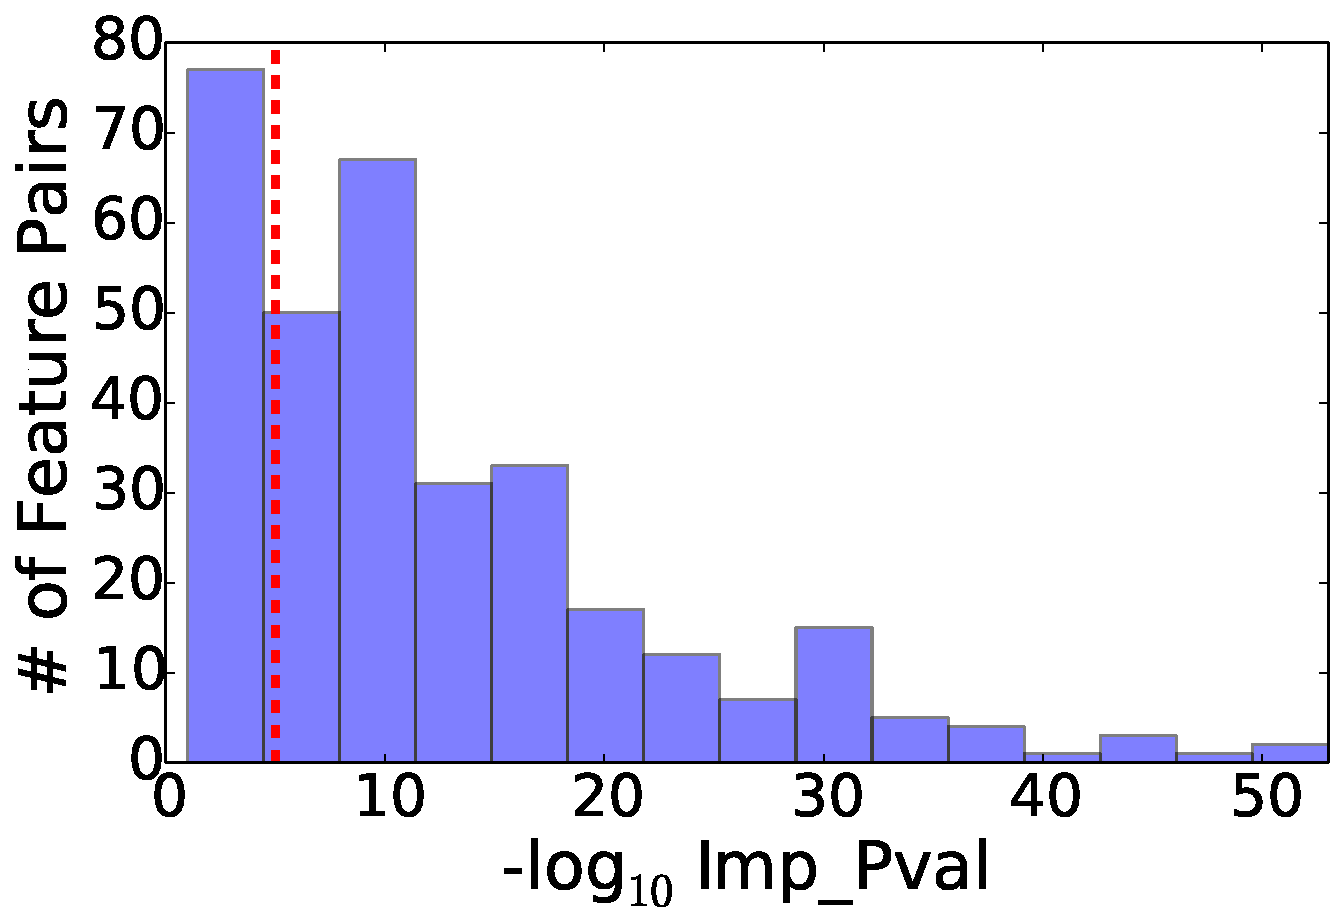
\includegraphics[width=.235\textwidth]{fig/histogram_lincs_diff_pval.pdf}}
\vspace{-5mm}
\caption{Histogram of $improv\_quot$. For the \toptwenty feature pairs from all runs from the (a) \msig and (b) \lincs datasets, distribution of the improvement of the feature pair significance over the corresponding single feature significance. The red line shows the significance threshold of 5.}
\vspace{-3mm}
\label{fig:histogram_diff}
\end{figure}
